% One-pager summary for Snaphomz trial
\documentclass[11pt]{article}
\usepackage[margin=0.8in]{geometry}
\usepackage{graphicx}
\usepackage{booktabs}
\usepackage{array}
\usepackage{hyperref}
\usepackage{enumitem}
\usepackage{xcolor}
\usepackage{multicol}
\usepackage[font=small,labelfont=bf]{caption}
\hypersetup{colorlinks=true, urlcolor=blue, linkcolor=blue}

\setlength{\parskip}{4pt}
\setlength{\parindent}{0pt}

\begin{document}

{\Large \textbf{Snaphomz Trial: EDA, Baseline Modeling, and Local RAG}}\\[4pt]
\textit{Notebook: notebooks/trial.ipynb \quad Data: data/listings\_sample.csv}

\vspace{0.5em}
\hrule\vspace{0.7em}

\section*{Highlights}
\begin{itemize}[leftmargin=*]
  \item No missing values in key fields; derived target \texttt{price\_per\_sqft}.
  \item Distributions for \texttt{price} and \texttt{sqft} are right-skewed; city medians show clear pps differences.
  \item Engineered features: keyword flags (pool/garage/quiet/updated/backyard), ratios, logs, and city priors.
  \item Baseline regression (test): \textbf{RandomForest} R$^2$ \(\approx 0.61\), better than Linear.
  \item LLM feature: local TF-IDF retriever + rule-based synthesis; returns answer with supporting contexts.
\end{itemize}

\section*{Key Metrics}
\vspace{-0.5em}
\begin{center}
\begin{tabular}{lccc}
\toprule
Model & MAE & RMSE & R$^2$ \\
\midrule
Linear Regression & 111.4 & 22746.9 & 0.584 \\
Random Forest Regressor & \textbf{107.9} & \textbf{21361.2} & \textbf{0.610} \\
\bottomrule
\end{tabular}
\end{center}

\vspace{0.4em}
\textbf{Takeaway:} size, city effects, and lightweight text features capture moderate signal; nonlinearity helps.

\section*{Representative Screenshots}
\vspace{-0.6em}
\begin{center}

\begin{minipage}[t]{0.48\linewidth}
  \centering
  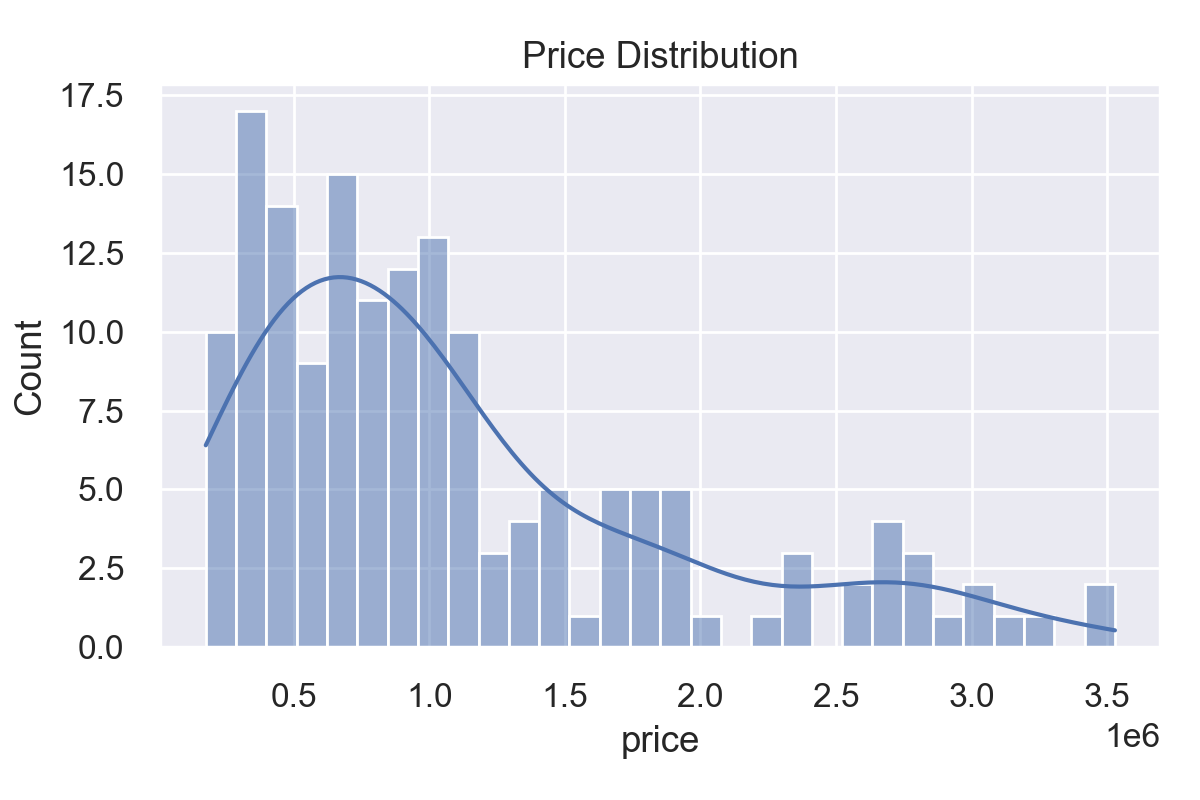
\includegraphics[width=\linewidth]{fig_price_dist.png}
  \captionof{figure}{Price distribution (right-skewed)}
\end{minipage}\hfill
\begin{minipage}[t]{0.48\linewidth}
  \centering
  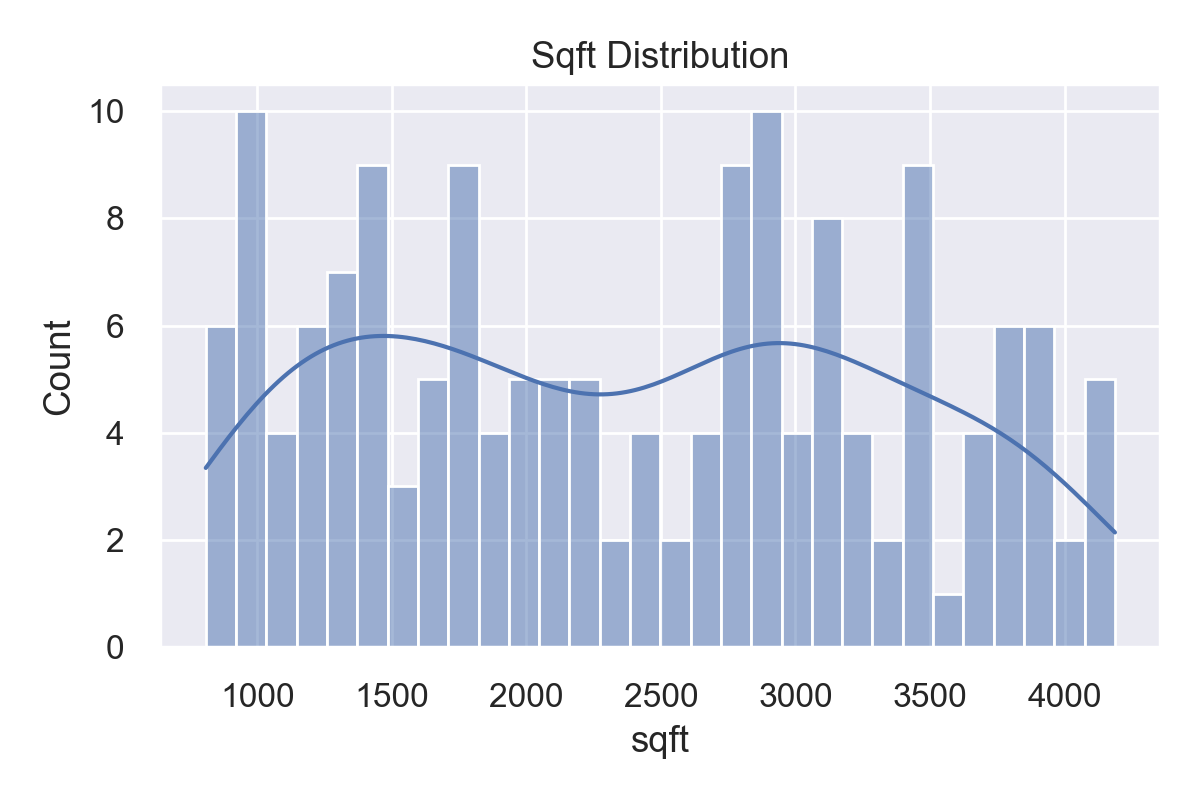
\includegraphics[width=\linewidth]{fig_sqft_dist.png}
  \captionof{figure}{Sqft distribution (right-skewed)}
\end{minipage}

\vspace{0.6em}

\begin{minipage}[t]{0.48\linewidth}
  \centering
  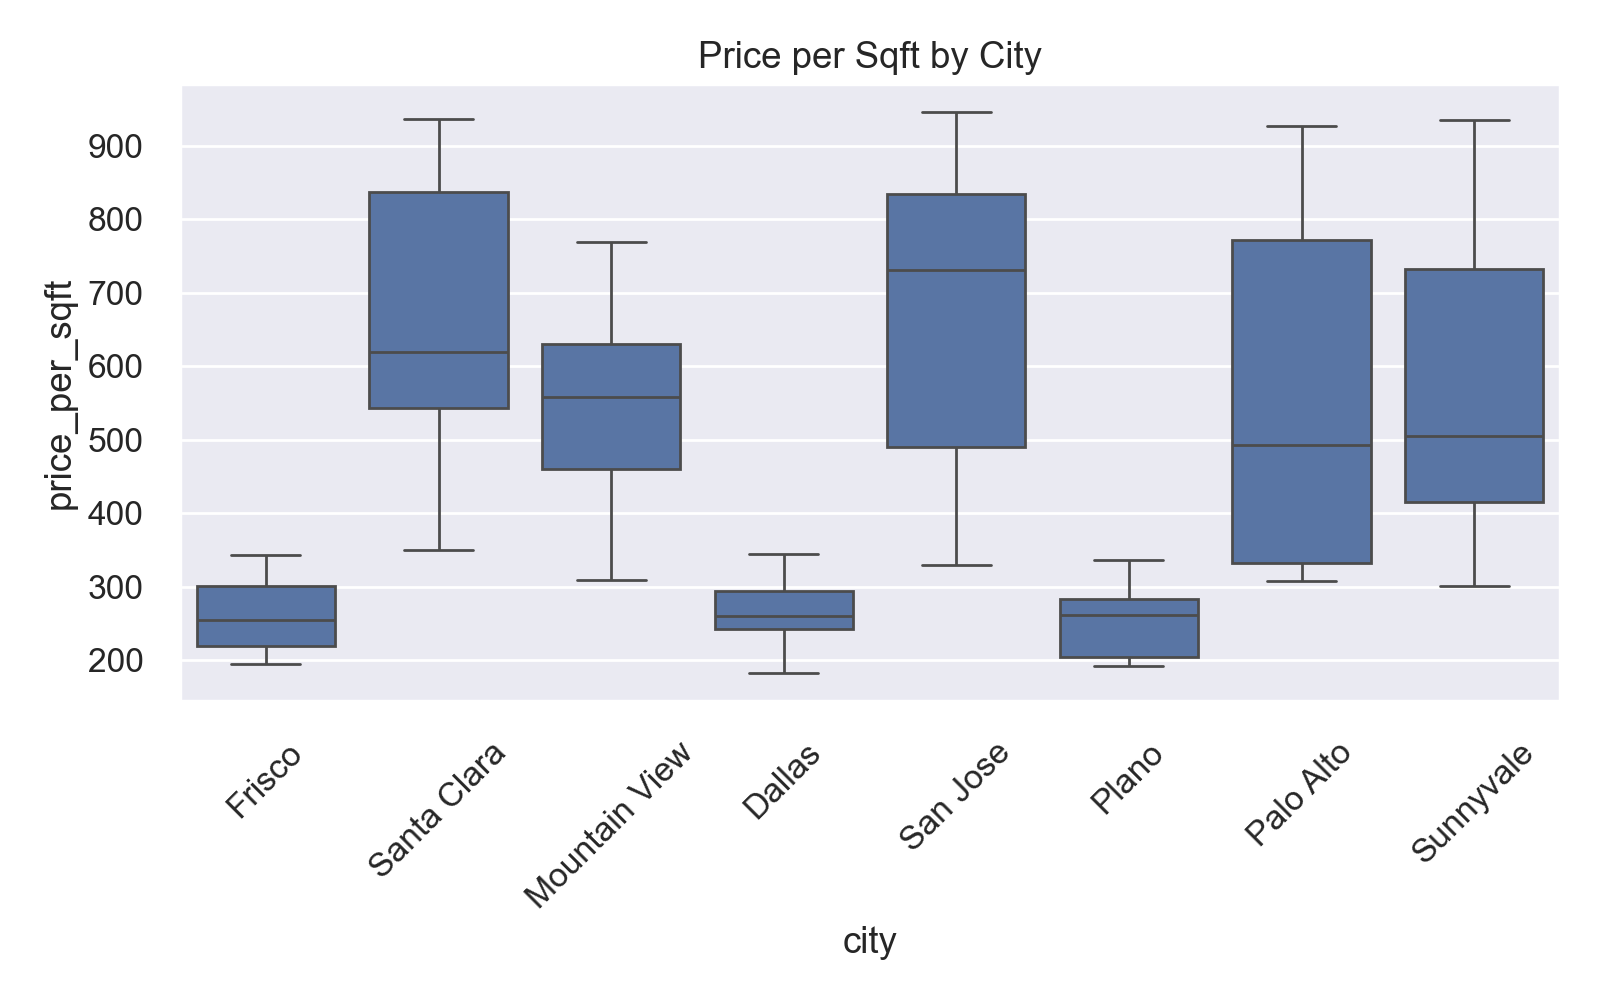
\includegraphics[width=\linewidth]{fig_pps_by_city.png}
  \captionof{figure}{Price per sqft by city (boxplot)}
\end{minipage}\hfill
\begin{minipage}[t]{0.48\linewidth}
  \centering
  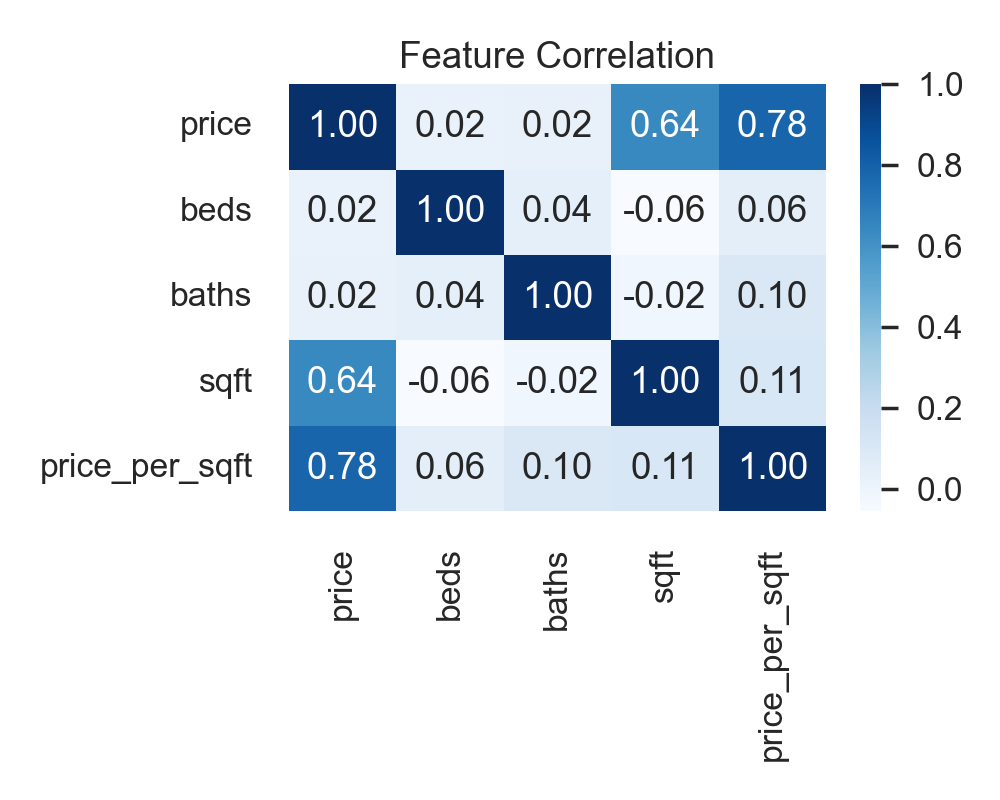
\includegraphics[width=\linewidth]{fig_corr_heatmap.png}
  \captionof{figure}{Correlation heatmap}
\end{minipage}

\end{center}

\section*{LLM Mini Q\&A (Local)}
\textbf{Retriever:} TF-IDF + NearestNeighbors (cosine).\\
\textbf{Answering:} Rule-based synthesis; returns short answer + top-k contexts (\texttt{id} + remark snippet).\\
\textbf{Example:}
\begin{quote}\small
Q: Do these listings typically have a pool?\\
A: Here is what I found from similar listings: Pool mentioned: yes.
\end{quote}

\section*{How to Reproduce}
\begin{enumerate}[leftmargin=*]
  \item Create and activate a virtual environment; install deps:
  \begin{quote}\small
  \texttt{python -m venv .venv \\ \&\& source .venv/bin/activate \\ \&\& pip install -r requirements.txt}
  \end{quote}
  \item Open and run \texttt{notebooks/trial.ipynb} from top to bottom.
  \item Export figures using the last cell (they will be saved to \texttt{results/}).
  \item Compile this one-pager to PDF:
  \begin{quote}\small
  \texttt{cd results \\ \&\& pdflatex one\_pager.tex}
  \end{quote}
\end{enumerate}

\section*{Notes \ \small (Limits \ \& Upgrades)}
\begin{itemize}[leftmargin=*]
  \item Small dataset; minimal tuning. Consider per-city models or interactions.
  \item Upgrade RAG: swap TF-IDF for open embeddings (e.g., BAAI/bge-small-en-v1.5) and optional reranker.
  \item Add local generation (e.g., FLAN-T5 small) for richer answers or 2--3 sentence summaries.
\end{itemize}

\vfill
\hrule
\small{Contact: KaheiLam/kaheilam973@gmail.com. Repo: https://github.com/Althealam/snaphomz-tria-KaheiLam}

\end{document}